% BIÊN DỊCH BẰNG XELATEX TRÊN OVERLEAF
\documentclass[14pt,a4paper]{extreport}

% ---------- Font & ngôn ngữ tiếng Việt ----------
\usepackage{fontspec}
\setmainfont{Liberation Serif}
\usepackage{polyglossia}
\setmainlanguage{vietnamese}

% ---------- Lề & giãn dòng ----------
\usepackage[a4paper,left=3cm,right=2cm,top=2.5cm,bottom=2.5cm]{geometry}
\usepackage{setspace}
\onehalfspacing

% ---------- Các gói hỗ trợ ----------
\usepackage{graphicx}
\usepackage{float}
\usepackage{array}
\usepackage{longtable}
\usepackage{booktabs}
\usepackage{multirow}
\usepackage{enumitem}
\usepackage{titlesec}
\usepackage{tikz}
\usetikzlibrary{positioning, fit, calc}
\usepackage{xcolor}
\usepackage{fancyhdr}
\usepackage[hidelinks]{hyperref}

% ---------- Định dạng mục lục & tiêu đề ----------
\renewcommand{\chaptername}{CHƯƠNG}
\renewcommand{\contentsname}{MỤC LỤC}
\renewcommand{\listfigurename}{DANH MỤC CÁC HÌNH VẼ}
\renewcommand{\listtablename}{DANH MỤC CÁC BẢNG}
\renewcommand{\figurename}{Hình}
\renewcommand{\tablename}{Bảng}

\titleformat{\chapter}[block]
  {\normalfont\Large\bfseries\centering}
  {\chaptertitlename\ \thechapter.}
  {0.5em}
  {\MakeUppercase}
\titlespacing*{\chapter}{0pt}{0pt}{24pt}

\titleformat{\section}
  {\normalfont\bfseries\large}{\thesection}{0.6em}{}
\titleformat{\subsection}
  {\normalfont\bfseries}{\thesubsection}{0.6em}{}

% ---------- Header/Footer ----------
\pagestyle{fancy}
\fancyhf{} 
\renewcommand{\headrulewidth}{0pt} 
\fancyfoot[C]{\thepage} 
\renewcommand{\chaptermark}[1]{}
\renewcommand{\sectionmark}[1]{}

% ---------- Cấu hình bảng & Macro tự tạo ----------
\newcolumntype{L}[1]{>{\raggedright\arraybackslash}p{#1}}
\setlist[itemize]{itemsep=2pt, topsep=3pt}

\newcommand{\anhplaceholder}[2]{%
  \begin{figure}[H]
    \centering
    \fbox{\parbox[c][6cm][c]{0.85\textwidth}{\centering
      \itshape \textcolor{red}{[TODO: Chèn ảnh thật tại đây --\\ #2]}}}
    \caption{#1}
  \end{figure}%
}

% ============================================================
\begin{document}

% ==================== TRANG BÌA ====================
\begin{titlepage}
\IfFileExists{khung.png}{%
\begin{tikzpicture}[remember picture, overlay]
    \node[inner sep=0pt] at (current page.center) {%
        
\includegraphics[width=18.5cm,height=27.5cm]{khung.png}%
    };
\end{tikzpicture}}{}

\begin{center}
\vspace*{-0.8cm}
{\large \textbf{HỌC VIỆN CÔNG NGHỆ BƯU CHÍNH VIỄN THÔNG}}\\[0.6cm]
{\large \textbf{KHOA KỸ THUẬT ĐIỆN TỬ 1}}\\[0.3cm]
\rule{6cm}{0.8pt}\\[0.5cm]

\IfFileExists{ptit_logo.png}{
\includegraphics[width=0.35\linewidth]{ptit_logo.png}\\[0cm]}{\vspace{3cm}}

{\LARGE\bfseries BÁO CÁO TIẾN ĐỘ LẦN 2 \\ ĐỒ ÁN TỐT NGHIỆP}\\[0.5cm]

{\large\itshape\bfseries Đề tài: Nghiên cứu, ứng dụng thuật toán Minimax \\ trong bài toán
ra quyết định và điều phối robot bầy đàn}\\[1.5cm] 

\renewcommand{\arraystretch}{1.3} 
{\large
\begin{tabular}{ll}
\textbf{Dương Sơn Quang}   & \textbf{MSV: B22DCDT238} \\
\textbf{Trương Hoàng Phúc} & \textbf{MSV: B22DCDT234} \\
\end{tabular}
}\\[1.5cm]

{\large \textbf{Giảng viên hướng dẫn: \hspace{0.2cm} TS. Phạm Hoàng Anh}}
\vfill
{\large \textbf{HÀ NỘI, 11/2026}}
\vspace*{-0.8cm}
\end{center}
\end{titlepage}

% ==================== MỤC LỤC ====================
\clearpage
\tableofcontents
\clearpage

% ==================== NỘI DUNG ====================
\pagenumbering{arabic}
\setcounter{page}{1}
 
\chapter*{1. TÓM TẮT TIẾN ĐỘ}
\addcontentsline{toc}{chapter}{1. TÓM TẮT TIẾN ĐỘ}
 
\begin{table}[H]
\renewcommand{\arraystretch}{1.3}
\begin{tabular}{@{}L{4.5cm} L{10cm}@{}}
\textbf{Đề tài} & Nghiên cứu, ứng dụng thuật toán Minimax trong bài toán ra quyết định và điều phối robot bầy đàn (mô hình Three Men's Morris) \\
\textbf{Thành viên} & Dương Sơn Quang (B22DCDT238)\\ & Trương Hoàng Phúc (B22DCDT234)\\ & Lớp: D22DTMT-01 -- Khóa: D22 \\
\textbf{GVHD} & TS. Phạm Hoàng Anh \\
\textbf{Kỳ báo cáo} & Lần 2 (15--25/11/2026); ngày lập báo cáo: \textbf{25/11/2026} \\
\textbf{Thời điểm kế hoạch} & Tuần \textbf{thứ 10} / 14 tuần (Hoàn thành Giai đoạn 1--4, đang triển khai Giai đoạn 5) \\
\end{tabular}
\end{table}
 
\subsection*{Tình hình chung}
Tính đến thời điểm báo cáo lần 2, nhóm đã hoàn tất toàn bộ \textbf{Giai đoạn 1 đến Giai đoạn 4} và hoàn thành phần lớn các hạng mục hiệu chỉnh độc lập của \textbf{Giai đoạn 5} theo đúng lộ trình 14 tuần trong Đề cương. Các phân hệ rời rạc ở báo cáo lần 1 nay đã được hoàn thiện và kiểm thử hoạt động ổn định trên từng khối chức năng.

Về \textbf{khối chấp hành và truyền thông (Tầng 2 \& Tầng 3)}, nhóm đã hoàn thiện phần cứng cơ khí và mạch điện tử cho cụm 6 xe robot tự hành (ESP32-WROOM-32D, mạch cầu H DRV8833, encoder, MPU6050, 5 mắt hồng ngoại TCRT5000L, dải LED WS2812B) cùng bộ điều phối trung gian (ESP32-WROOM-32 DevKit chạy 5 tác vụ FreeRTOS). Phần mềm nhúng trên xe đã hoàn thiện bộ điều khiển \textbf{PID dò line} chạy ổn định, đọc chính xác góc quay từ \textbf{MPU6050} và thông suốt giao tiếp không dây hai chiều qua \textbf{ESP-NOW} giữa các xe với khối xử lý trung tâm.

Về \textbf{khối xử lý trung tâm và giao diện (Tầng 1)}, nhóm đã hoàn thiện giao diện \textbf{Web Dashboard} (React/TypeScript), máy chủ WebSocket, dịch vụ thị giác máy tính (\texttt{camera\_service.py}) và bộ giải thuật \textbf{AI Minimax} (\texttt{minimax.py}). Hệ thống đã hiệu chỉnh xong Camera, nắn phẳng bàn cờ bằng ma trận biến đổi đồng ứng (Homography) và nhận diện ổn định tọa độ, góc hướng của các quân cờ/xe robot thông qua thẻ \textbf{ArUco} kết hợp cảm biến \textbf{MPU6050}. Thuật toán Minimax hoạt động chính xác, đưa ra nước đi tối ưu theo thời gian thực.

\subsection*{Những việc đã hoàn thành chính (từ sau lần 1)}
\begin{enumerate}
    \item \textbf{Hoàn thiện phần cứng hệ thống:} Gia công PCB, hàn lắp và kiểm thử cơ khí, mạch nguồn, mạch động lực cho cụm 6 xe robot tự hành và mạch điều phối trung gian ESP32-WROOM-32 DevKit; hệ thống chạy ổn định, không sụt áp hay treo vi điều khiển.
    \item \textbf{Hoàn thiện giao diện Web và máy chủ điều khiển:} Xây dựng hoàn chỉnh Web Dashboard (React/TypeScript) kết nối WebSocket thời gian thực với backend Python, hỗ trợ đầy đủ chế độ mô phỏng ván đấu và bảng kiểm tra trước vận hành (Pre-Flight Check).
    \item \textbf{Hoàn thiện thuật toán AI Minimax và quy hoạch quỹ đạo:} Cài đặt hoàn chỉnh thuật toán Minimax (độ sâu $d=4$, cắt tỉa Alpha-Beta, Transposition Table) có khả năng phản hồi nước cờ tối ưu tức thì; tích hợp bộ lập kế hoạch quỹ đạo BFS/A* (\texttt{board\_planner.py}), vượt qua 44/44 bài kiểm thử đơn vị (unit test).
    \item \textbf{Hoàn thiện dịch vụ thị giác máy tính và hiệu chỉnh Camera:} Thu hình MJPG $640\times480$ ở 30 fps không trễ; hoàn tất hiệu chỉnh Homography qua 4 thẻ mốc ArUco góc bàn cờ (\texttt{DICT\_5X5\_100}, ID 90--93), lưu cấu hình \texttt{camera\_calibration.json}; nhận diện chính xác vị trí và góc hướng của các thẻ xe (ID 1--6).
    \item \textbf{Hoàn thiện điều khiển chuyển động và định vị trên xe:} Lập trình nhúng hoàn chỉnh điều khiển động cơ PWM 20 kHz, đếm xung encoder, đọc góc quay từ cảm biến quán tính \textbf{MPU6050} và hoàn thiện bộ điều khiển \textbf{PID dò line} thích nghi với 5 cảm biến hồng ngoại TCRT5000L giúp xe bám vạch mượt, hết dao động.
    \item \textbf{Hoàn thiện truyền thông ESP-NOW:} Tổ chức 5 tác vụ FreeRTOS trên Coordinator, giao tiếp UART2 và truyền nhận gói tin nhị phân hai chiều (\texttt{RobotCmdPacket}, \texttt{RobotLedPacket}, \texttt{RobotStatusPacket}) ổn định giữa khối trung tâm và các xe.
\end{enumerate}

\subsection*{Những việc sắp làm (Hoàn thiện Giai đoạn 5 \& Giai đoạn 6)}
\begin{enumerate}
    \item \textbf{Kết hợp toàn diện hệ thống (End-to-End Integration):} Ghép nối khép kín luồng dữ liệu từ Camera (ArUco) $\rightarrow$ AI Minimax $\rightarrow$ Lập kế hoạch quỹ đạo BFS/A* $\rightarrow$ ESP-NOW $\rightarrow$ Cụm 6 xe thực thi nước đi đồng bộ trên sa bàn thực tế.
    \item \textbf{Tối ưu chương trình di chuyển trên bàn cờ:} Tinh chỉnh tham số chuyển tiếp giữa các pha điều khiển (quay tại chỗ theo góc MPU6050/ArUco $\rightarrow$ chạy bám vạch bằng PID $\rightarrow$ giảm tốc tuyến tính và dừng chính xác tại tâm nút giao) để xe di chuyển qua lại giữa các vị trí trên bàn cờ và bãi đỗ mượt mà nhất.
    \item \textbf{Thu thập số liệu và hoàn thiện báo cáo:} Đo đạc sai số định vị, thời gian phản hồi, tỷ lệ thực thi nước đi thành công của toàn hệ thống để hoàn thiện quyển báo cáo Đồ án tốt nghiệp và slide bảo vệ.
\end{enumerate}
 
\subsection*{Vấn đề kỹ thuật cần lưu ý trong giai đoạn tích hợp}
\begin{itemize}
    \item Đồng bộ hóa thời gian thực giữa tọa độ phản hồi từ Camera trên cao (ArUco) và tọa độ ước lượng cục bộ trên xe (Encoder + MPU6050 + dò vạch) khi nhiều xe cùng thực hiện thao tác nhường đường trên không gian bàn cờ hẹp.
    \item Tinh chỉnh ngưỡng giảm tốc khi xe tiếp cận tâm nút giao để triệt tiêu hoàn toàn quán tính trượt cơ khí, đảm bảo độ mượt và độ lặp lại cao qua nhiều lượt đi liên tiếp.
\end{itemize}

\chapter*{2. TỔNG QUAN KIẾN TRÚC HỆ THỐNG}
\addcontentsline{toc}{chapter}{2. TỔNG QUAN KIẾN TRÚC HỆ THỐNG}
 
Hệ thống được thiết kế theo kiến trúc phân tầng ba lớp rõ rệt: (1) \textbf{Tầng chiến lược, thị giác và điều phối cấp cao} (Raspberry Pi 3 + Camera USB) đảm nhiệm xử lý ảnh OpenCV nhận diện ArUco, AI Minimax, quy hoạch quỹ đạo BFS/A* và Web Server; (2) \textbf{Tầng cầu nối chuyển tiếp thời gian thực} (mạch ESP32-WROOM-32 DevKit chạy FreeRTOS) nhận lệnh qua UART2 và phát xuống các xe bằng giao thức nhị phân ESP-NOW; (3) \textbf{Tầng chấp hành và định vị cục bộ} gồm 6 xe robot tự hành (ESP32-WROOM-32D) điều khiển chuyển động lai kết hợp PID dò line, encoder và MPU6050.
 
\begin{figure}[H]
\centering
\begin{tikzpicture}[
  box/.style={draw, rounded corners=3pt, align=center, font=\footnotesize, minimum height=1.3cm, text width=2.8cm},
  arr/.style={-stealth, thick},
  lab/.style={font=\scriptsize\itshape, fill=white, inner sep=1pt}]

  % Khởi tạo các khối chính
  \node[box] (cam) {Camera USB\\thu ảnh sa bàn};
  \node[box, right=1.2cm of cam] (pi) {Raspberry Pi 3\\OpenCV, Minimax,\\ BFS/A*, Web Server};
  \node[box, right=1.2cm of pi] (co) {ESP32 DevKit\\Coordinator\\(FreeRTOS)};
  \node[box, right=1.2cm of co] (car) {6 xe tự hành\\ESP32 + PID dò line\\+ MPU6050};
  
  % Khối Web Dashboard được đặt lên trên khối Raspberry Pi
  \node[box, above=1.2cm of pi] (web) {Trình duyệt\\(Web Dashboard)};

  % Kết nối các khối ngang
  \draw[arr] (cam) -- (pi);
  \draw[arr] (pi) -- node[above, lab]{UART2} (co);
  \draw[arr] (co) -- node[above, lab]{ESP-NOW} (car);
  
  % Vòng phản hồi từ xe về camera (đi vòng xuống dưới)
  \draw[arr] (car.south) -- ++(0,-1) -| node[pos=0.25, below, lab]{Phản hồi vị trí \& góc (ArUco)} (cam.south);
  
  % Kết nối giao tiếp với Web (hướng lên trên)
  \draw[arr, <->] (pi) -- node[right, lab]{WebSocket} (web);

\end{tikzpicture}
\vspace{0.5cm}
\caption{Sơ đồ khối kiến trúc phân tầng ba lớp của hệ thống.}
\label{fig:sodokhoi}
\end{figure}
 
\textbf{Luồng hoạt động một nước đi:} Camera nhận diện trạng thái bàn cờ và góc/vị trí xe qua ArUco $\rightarrow$ Minimax chọn quân cờ và ô đích tối ưu $\rightarrow$ Bộ lập kế hoạch quỹ đạo (BFS giải phóng nút cản + $A^*$ tìm đường) tạo danh sách waypoint $\rightarrow$ Gửi tuần tự qua UART2 và ESP-NOW $\rightarrow$ Xe thực thi bám quỹ đạo (MPU6050 + PID dò line), dừng tại ô đích $\rightarrow$ Camera xác nhận, cập nhật trạng thái lên Web Dashboard.

\textbf{Hiện trạng:} Đến thời điểm báo cáo lần 2, toàn bộ các phân hệ ở cả 3 tầng đã được xây dựng và kiểm thử hoạt động ổn định độc lập; nhóm đang bước vào công đoạn ghép nối tổng thể và tối ưu chuyển động di chuyển liên tục trên bàn cờ.
 
% ============================================================
\chapter*{3. ĐỐI CHIẾU KẾ HOẠCH VÀ THỰC TẾ}
\addcontentsline{toc}{chapter}{3. ĐỐI CHIẾU KẾ HOẠCH VÀ THỰC TẾ}
 
Bảng 1 đối chiếu tiến độ thực tế của nhóm với lộ trình 14 tuần (chia thành các hạng mục chi tiết thuộc 6 giai đoạn triển khai) trong Đề cương Đồ án tốt nghiệp.
 
\begin{longtable}{c L{6.2cm} L{2.0cm} c L{2.6cm}}
\caption{Đối chiếu tiến độ thực tế với Đề cương}\label{tab:doichieu}\\
\toprule
\textbf{ID} & \textbf{Công việc} & \textbf{Phụ trách} & \textbf{Tuần KH} & \textbf{Trạng thái} \\
\midrule\endfirsthead
\toprule
\textbf{ID} & \textbf{Công việc} & \textbf{Phụ trách} & \textbf{Tuần KH} & \textbf{Trạng thái} \\
\midrule\endhead
 
\midrule \multicolumn{5}{l}{\textbf{Giai đoạn 1: Nghiên cứu và thiết kế tổng thể (Tuần 1--2)}}\\
1 & Nghiên cứu lý thuyết Minimax, điều phối bầy đàn & Cả 2 & 1--2 & \textbf{Hoàn thành} \\
2 & Thiết kế kiến trúc tổng thể phân tầng 3 lớp & Cả 2 & 1--2 & \textbf{Hoàn thành} \\
3 & Chọn linh kiện, lập bảng phân chân và BOM & Cả 2 & 2 & \textbf{Hoàn thành} \\
 
\midrule \multicolumn{5}{l}{\textbf{Giai đoạn 2: Thiết kế, chế tạo phần cứng (Tuần 3--5)}}\\
4 & Thiết kế mạch nguyên lý (Schematic) & Phúc & 3 & \textbf{Hoàn thành} \\
5 & Thiết kế mạch in PCB: driver DRV8833, nguồn, cảm biến & Phúc & 3--4 & \textbf{Hoàn thành} \\
6 & Gia công cơ khí, lắp ráp hoàn thiện 6 xe robot & Phúc & 4--5 & \textbf{Hoàn thành} \\
7 & Lắp ráp mạch điều phối ESP32-WROOM-32 DevKit & Quang & 4--5 & \textbf{Hoàn thành} \\
 
\midrule \multicolumn{5}{l}{\textbf{Giai đoạn 3: Phần mềm trung tâm, AI, Thị giác máy tính \& Web (Tuần 5--7)}}\\
8 & Mô hình hóa bàn cờ 9 nút & Quang & 5 & \textbf{Hoàn thành} \\
9 & Thuật toán AI Minimax cắt tỉa Alpha-Beta (\texttt{minimax.py}) & Quang & 5--6 & \textbf{Hoàn thành} \\
10 & Quy hoạch quỹ đạo BFS và $A^*$ (\texttt{board\_planner.py}) & Quang & 6--7 & \textbf{Hoàn thành} \\
11 & Dịch vụ thị giác máy tính ArUco, Homography (\texttt{camera\_service.py}) & Quang & 6--7 & \textbf{Hoàn thành} \\
12 & Giao diện Web Dashboard (React/TypeScript) \& WebSocket & Quang & 6--7 & \textbf{Hoàn thành} \\
 
\midrule \multicolumn{5}{l}{\textbf{Giai đoạn 4: Lập trình nhúng FreeRTOS, ESP-NOW \& Điều khiển xe (Tuần 7--9)}}\\
13 & Lập trình FreeRTOS (5 task) \& UART2 cho Coordinator & Quang & 7--8 & \textbf{Hoàn thành} \\
14 & Giao tiếp nhị phân ESP-NOW hai chiều (Coordinator $\leftrightarrow$ 6 xe) & Cả 2 & 7--8 & \textbf{Hoàn thành} \\
15 & Điều khiển động cơ PWM 20 kHz, đọc Encoder \& MPU6050 & Phúc & 7--8 & \textbf{Hoàn thành} \\
16 & Thuật toán PID dò line thích nghi (5 mắt TCRT5000L) & Phúc & 8--9 & \textbf{Hoàn thành} \\
 
\midrule \multicolumn{5}{l}{\textbf{Giai đoạn 5: Tích hợp hệ thống \& Tinh chỉnh quỹ đạo (Tuần 10--12)}}\\
17 & Hiệu chỉnh camera, nhận diện góc và vị trí quân cờ ArUco & Quang & 10 & \textbf{Hoàn thành} \\
18 & Tích hợp toàn hệ thống (Camera -- AI -- ESP-NOW -- 6 xe) & Cả 2 & 10--11 & \textbf{Đang triển khai} \\
19 & Tối ưu chương trình di chuyển giữa các ô cờ mượt mà & Phúc & 11--12 & \textbf{Đang triển khai} \\
 
\midrule \multicolumn{5}{l}{\textbf{Giai đoạn 6: Thực nghiệm, viết báo cáo và bảo vệ (Tuần 12--14)}}\\
20--22 & Thu thập số liệu thực nghiệm, viết quyển ĐATN, làm slide bảo vệ & Cả 2 & 12--14 & Chưa tới hạn \\
\bottomrule
\end{longtable}
 
\textbf{Nhận xét:} Toàn bộ các hạng mục từ Giai đoạn 1 đến Giai đoạn 4 đã hoàn thành đúng tiến độ đề ra. Phần cứng 6 xe vận hành ổn định; các khối phần mềm cốt lõi (Web, Minimax, Camera ArUco, ESP-NOW, PID dò line và cảm biến MPU6050) đều đã hoạt động tốt, tạo nền tảng vững chắc để nhóm tập trung hoàn toàn vào việc ghép nối hệ thống và tối ưu quỹ đạo di chuyển trong Giai đoạn 5.
 
% ============================================================
\chapter*{4. KẾT QUẢ ĐÃ ĐẠT}
\addcontentsline{toc}{chapter}{4. KẾT QUẢ ĐÃ ĐẠT}
 
\section*{4.1 Chế tạo và hoàn thiện phần cứng 6 xe tự hành}
Nhóm đã hoàn tất gia công PCB, hàn lắp linh kiện và lắp ráp cơ khí hoàn chỉnh cụm 6 xe robot vi sai hai bánh (bán kính bánh 30 mm, khoảng cách hai bánh 100 mm) cùng mạch điều phối trung gian ESP32-WROOM-32 DevKit. Mỗi xe sử dụng vi điều khiển ESP32-WROOM-32D, mạch cầu H DRV8833 (xung PWM 20 kHz), nguồn nuôi cách ly nhiễu giữa khối động lực và vi điều khiển, tích hợp encoder hai kênh, cảm biến quán tính MPU6050 (I2C), mảng 5 cảm biến hồng ngoại TCRT5000L (qua cầu phân áp vào ADC1) và dải 5 LED trạng thái WS2812B. Qua kiểm thử vận hành độc lập, phần cứng cả 6 xe hoạt động ổn định, không xảy ra hiện tượng sụt áp hay reset ngoài ý muốn.
 
\begin{figure}[H]
    \centering
    \IfFileExists{xe1.png}{\includegraphics[width=0.8\linewidth]{xe1.png}}{\fbox{\parbox[c][4cm][c]{0.8\textwidth}{\centering \itshape \textcolor{red}{[Thiếu file xe1.png]}}}}
    \caption{Một xe tự hành sau khi lắp ráp hoàn chỉnh}
    \label{fig:xe1}
\end{figure}
\begin{figure}[H]
    \centering
    \IfFileExists{xe6.png}{\includegraphics[width=0.8\linewidth]{xe6.png}}{\fbox{\parbox[c][4cm][c]{0.8\textwidth}{\centering \itshape \textcolor{red}{[Thiếu file xe6.png]}}}}
    \caption{Cụm sáu xe tự hành trên sa bàn cờ ba quân}
    \label{fig:xe6}
\end{figure}
 
\section*{4.2 Hệ thống xử lý trung tâm và giao tiếp truyền thông}
Phần mềm điều khiển trung tâm được phát triển bằng Python theo kiến trúc lập trình bất đồng bộ (\texttt{asyncio}), vận hành ổn định và liên kết thông suốt giữa ba dịch vụ cốt lõi: dịch vụ thị giác máy tính (\texttt{camera\_service.py}), máy chủ WebSocket giao tiếp với Web Dashboard và trình quản lý giao tiếp nối tiếp (\texttt{serial\_coordinator.py}) kết nối UART2 tốc độ 115200 bps tới bộ điều phối trung gian.

Trên tầng cầu nối, mạch ESP32-WROOM-32 DevKit tổ chức 5 tác vụ độc lập trên hệ điều hành thời gian thực FreeRTOS (\texttt{uart\_rx}, \texttt{uart\_tx}, \texttt{cmd\_hdlr}, \texttt{robot\_stat}, \texttt{heartbeat}), khóa cứng kênh vô tuyến số 1 và đăng ký sẵn địa chỉ MAC của 6 xe. Giao tiếp không dây hai chiều qua giao thức \textbf{ESP-NOW} (sử dụng các gói tin nhị phân cố định \texttt{RobotCmdPacket} 18 byte, \texttt{RobotLedPacket} 18 byte và \texttt{RobotStatusPacket} 8 byte) đã hoạt động thông suốt, phản hồi PING/PONG nhanh và không mất gói tin khi truyền nhận lệnh giữa khối trung tâm và các xe.

\section*{4.3 Xử lý ảnh, hiệu chỉnh Camera và nhận diện ArUco}
Dịch vụ thị giác máy tính (\texttt{camera\_service.py}) thu nhận khung hình từ camera USB ở định dạng MJPG độ phân giải $640\times480$ tại 30 fps bằng luồng đọc riêng biệt, phát video trực tiếp và ảnh nắn phẳng qua giao thức HTTP tại cổng 8080.

Nhóm đã hoàn thành quá trình \textbf{hiệu chỉnh Camera} sử dụng 4 thẻ mốc chuẩn ArUco (\texttt{DICT\_5X5\_100}, mã ID 90, 91, 92, 93) đặt tại bốn góc sa bàn. Hệ thống lấy giá trị trung vị qua 15 khung hình liên tiếp để tính ma trận biến đổi đồng ứng (Homography), ánh xạ vùng bàn cờ về mặt phẳng chuẩn hóa kích thước $800\times800$ pixel và lưu thông số vào tệp \texttt{camera\_calibration.json}. Trên mặt phẳng đã hiệu chỉnh, dịch vụ nhận diện ổn định các thẻ ArUco gắn trên nóc xe (ID 1--6), trích xuất chính xác tọa độ tâm $(x_b, y_b)$ và góc phương vị của từng quân cờ theo thời gian thực.
 
\begin{figure}[H]
    \centering
    \IfFileExists{camera_video.png}{\includegraphics[width=0.85\linewidth]{camera_video.png}}{\fbox{\parbox[c][4cm][c]{0.8\textwidth}{\centering \itshape \textcolor{red}{[Thiếu file camera\_video.png]}}}}
    \caption{Video camera nhận diện khung marker và trạng thái hiệu chuẩn}
    \label{fig:camvideo}
\end{figure}
\begin{figure}[H]
    \centering
    \IfFileExists{camera_warped.png}{\includegraphics[width=0.85\linewidth]{camera_warped.png}}{\fbox{\parbox[c][4cm][c]{0.8\textwidth}{\centering \itshape \textcolor{red}{[Thiếu file camera\_warped.png]}}}}
    \caption{Ảnh bàn cờ sau khi nắn phẳng chuẩn hóa $800\times800$ pixel}
    \label{fig:camwarped}
\end{figure}
 
\section*{4.4 Thuật toán ra quyết định Minimax và quy hoạch quỹ đạo}
Không gian hoạt động của trò chơi Three Men's Morris được mô hình hóa thành đồ thị vô hướng gồm 9 nút giao chiến lược (ID 0--8) và 2 khu vực bãi đỗ ở hai biên. Bộ giải thuật AI (\texttt{minimax.py}) cài đặt thuật toán tìm kiếm đối kháng Minimax với độ sâu tìm kiếm mặc định $d = 4$, tích hợp kỹ thuật cắt tỉa Alpha-Beta, bảng băm chuyển vị (Transposition Table) và sắp xếp thứ tự nước đi.

Qua kiểm thử thực tế và 44/44 bài kiểm thử đơn vị tự động, thuật toán Minimax hoạt động ổn định, đánh giá chính xác thế cờ trong cả hai giai đoạn Đặt quân (Placement Phase) và Di chuyển (Movement Phase), luôn đưa ra nước cờ tối ưu (chủ động tạo hàng 3 quân thẳng hàng hoặc chặn nước thắng của đối phương) với thời gian phản hồi tức thì. Song song đó, mô-đun \texttt{board\_planner.py} kết hợp thuật toán BFS (tìm nút trống lân cận giải phóng xe cản đường) và thuật toán $A^*$ để sinh chuỗi tọa độ waypoint không va chạm.
 
\begin{table}[H]
\centering
\caption{Kết quả kiểm thử các kịch bản tiêu biểu của thuật toán Minimax}
\begin{tabular}{L{4.5cm} L{4.5cm} c c}
\toprule
\textbf{Trạng thái bàn cờ đầu vào} & \textbf{Nước đi Minimax lựa chọn} & \textbf{Đánh giá} & \textbf{Thời gian} \\
\midrule
Người chơi có 2 quân thẳng hàng (sắp tạo Mill) & Điều phối xe vào ô trống thứ 3 để chặn nước thắng & Tối ưu & $< 15\text{ ms}$ \\
AI có cơ hội tạo thành 3 quân thẳng hàng & Điều phối xe vào ô hoàn thành hàng thắng & Tối ưu & $< 15\text{ ms}$ \\
Trạng thái khởi đầu giai đoạn đặt quân & Ưu tiên chiếm giữ nút trung tâm (nút số 4) & Tối ưu & $< 20\text{ ms}$ \\
\bottomrule
\end{tabular}
\end{table}
 
\section*{4.5 Giao diện giám sát Web Dashboard}
Nhóm đã hoàn thiện giao diện điều khiển Web bằng React và TypeScript, kết nối hai chiều theo thời gian thực tới máy chủ backend qua giao thức WebSocket. Giao diện đáp ứng đầy đủ hai chế độ vận hành: chế độ mô phỏng kiểm thử toàn ván đấu với AI Minimax và chế độ vận hành phần cứng thực tế tích hợp bảng kiểm tra trước vận hành (Pre-Flight Check), hiển thị luồng video trực tiếp từ camera, ảnh bàn cờ đã nắn phẳng cùng vị trí và góc hướng của cả 6 xe.
 
\begin{figure}[H]
    \centering
    \IfFileExists{web.png}{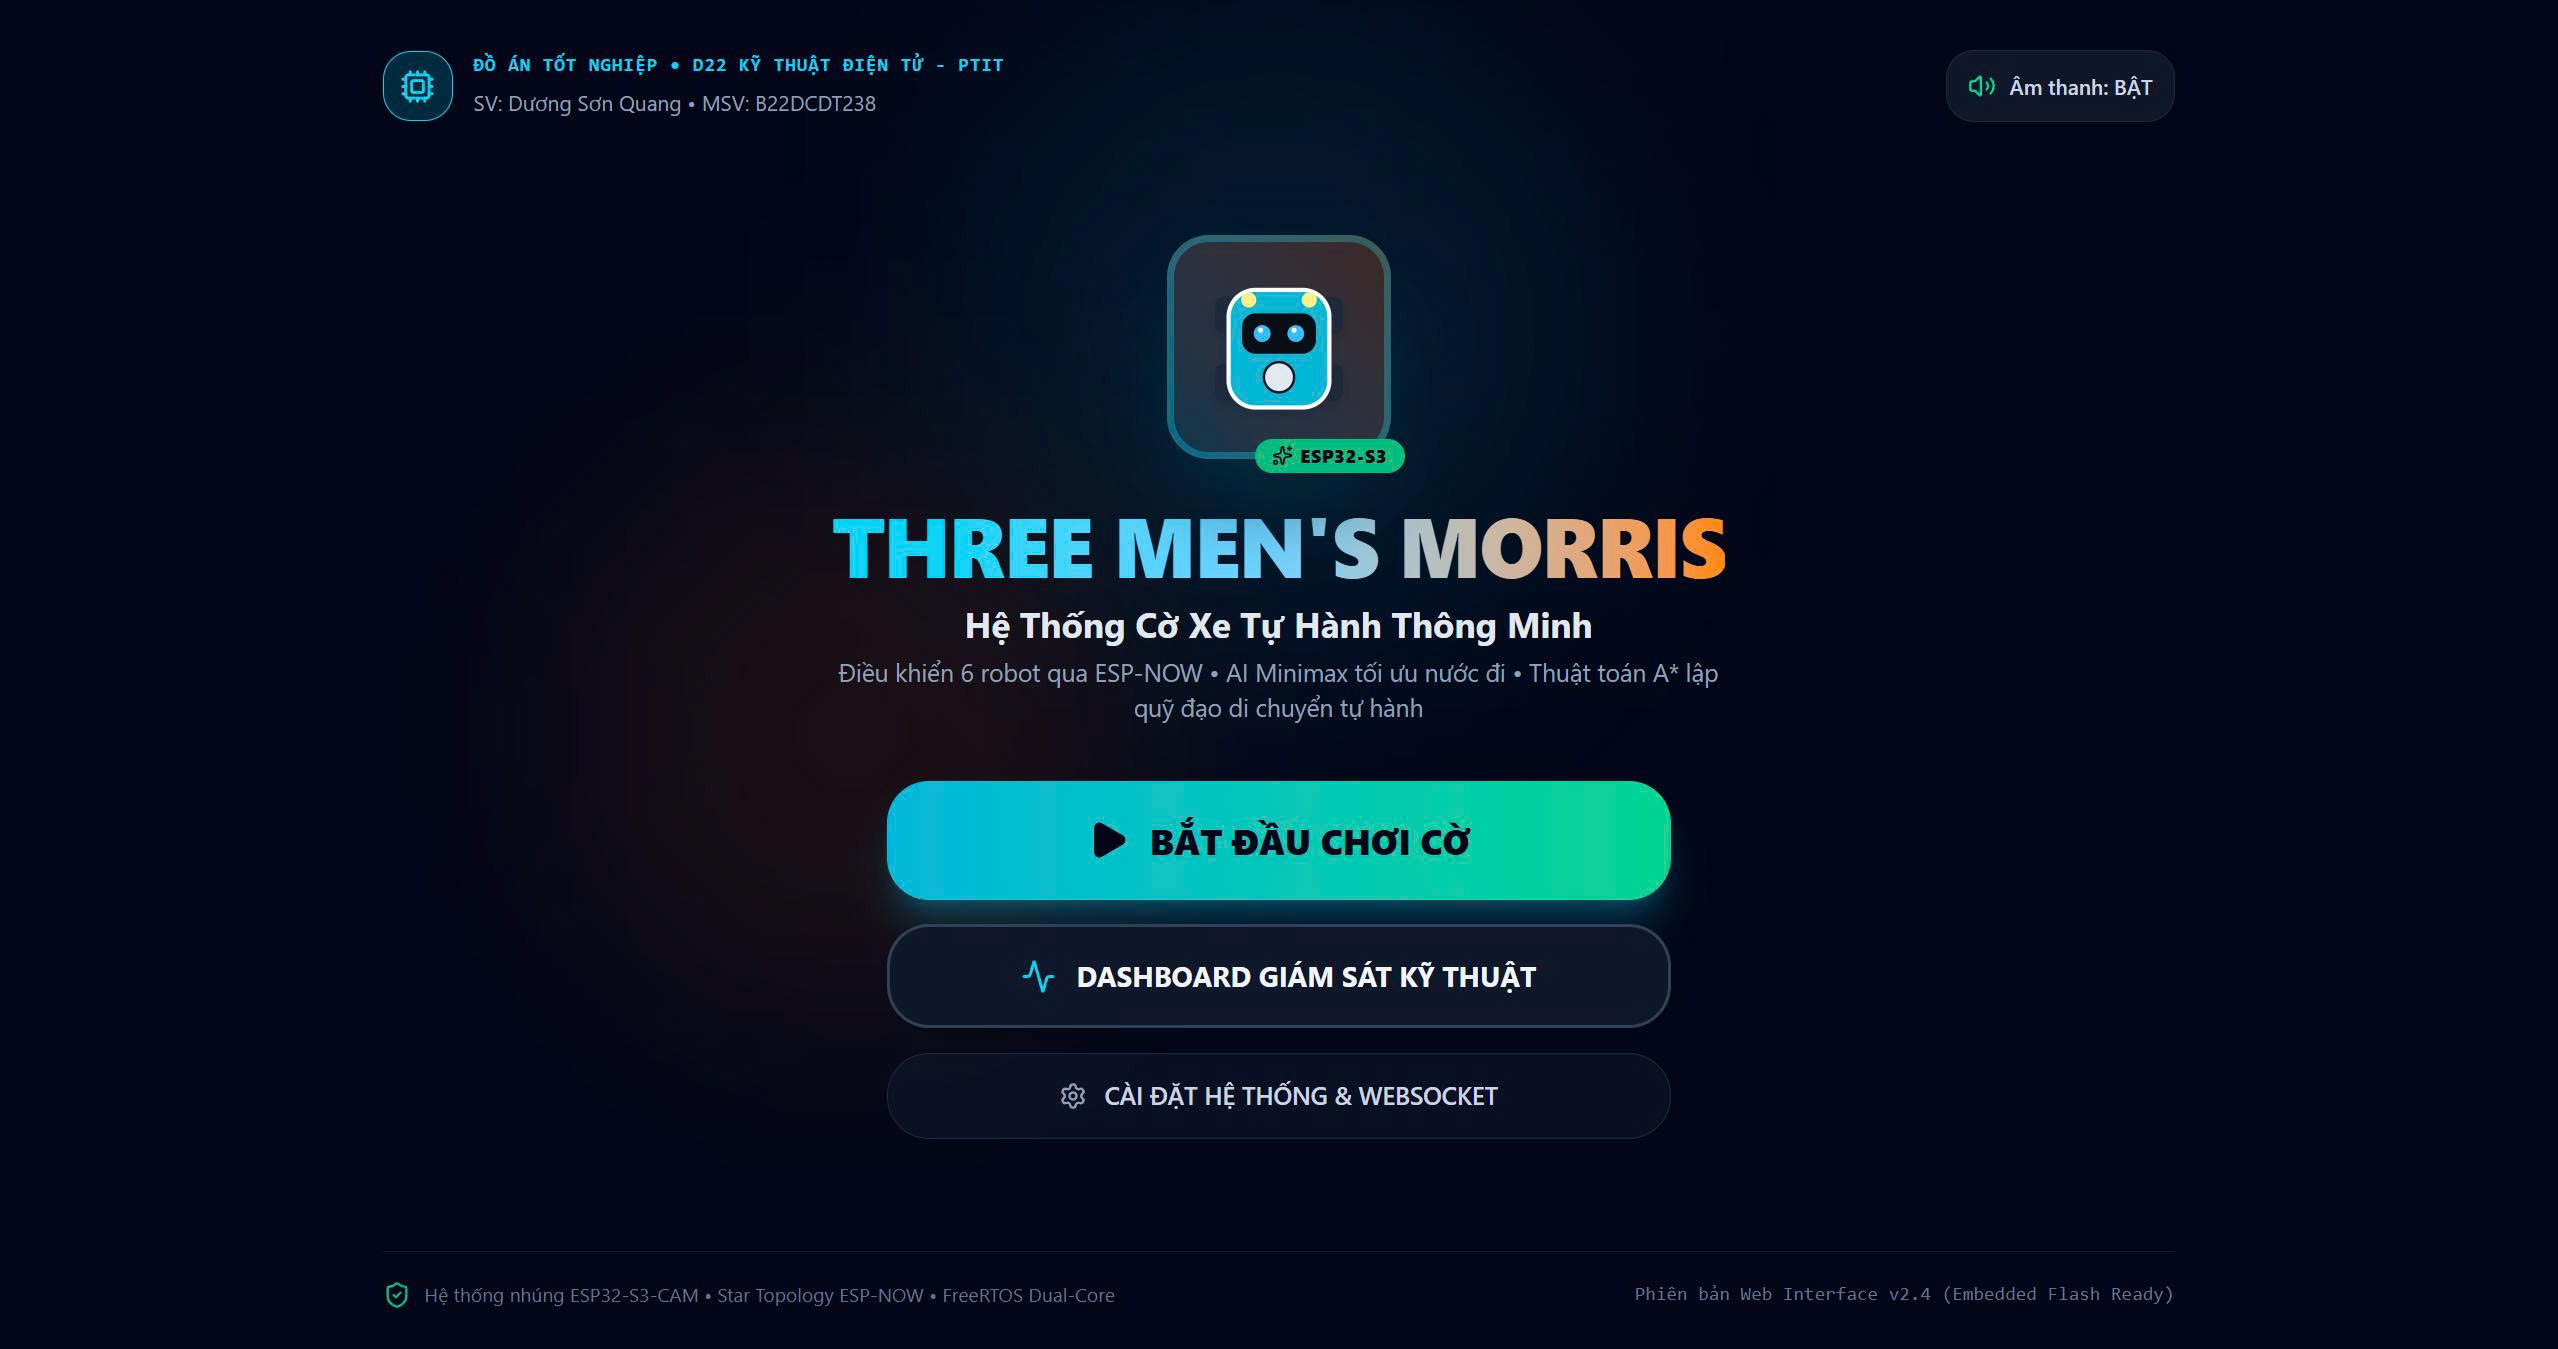
\includegraphics[width=0.95\linewidth]{web.png}}{\fbox{\parbox[c][4cm][c]{0.8\textwidth}{\centering \itshape \textcolor{red}{[Thiếu file web.png]}}}}
    \caption{Giao diện giám sát tổng thể Web Dashboard}
    \label{fig:web}
\end{figure}
\begin{figure}[H]
    \centering
    \IfFileExists{vitrixe.png}{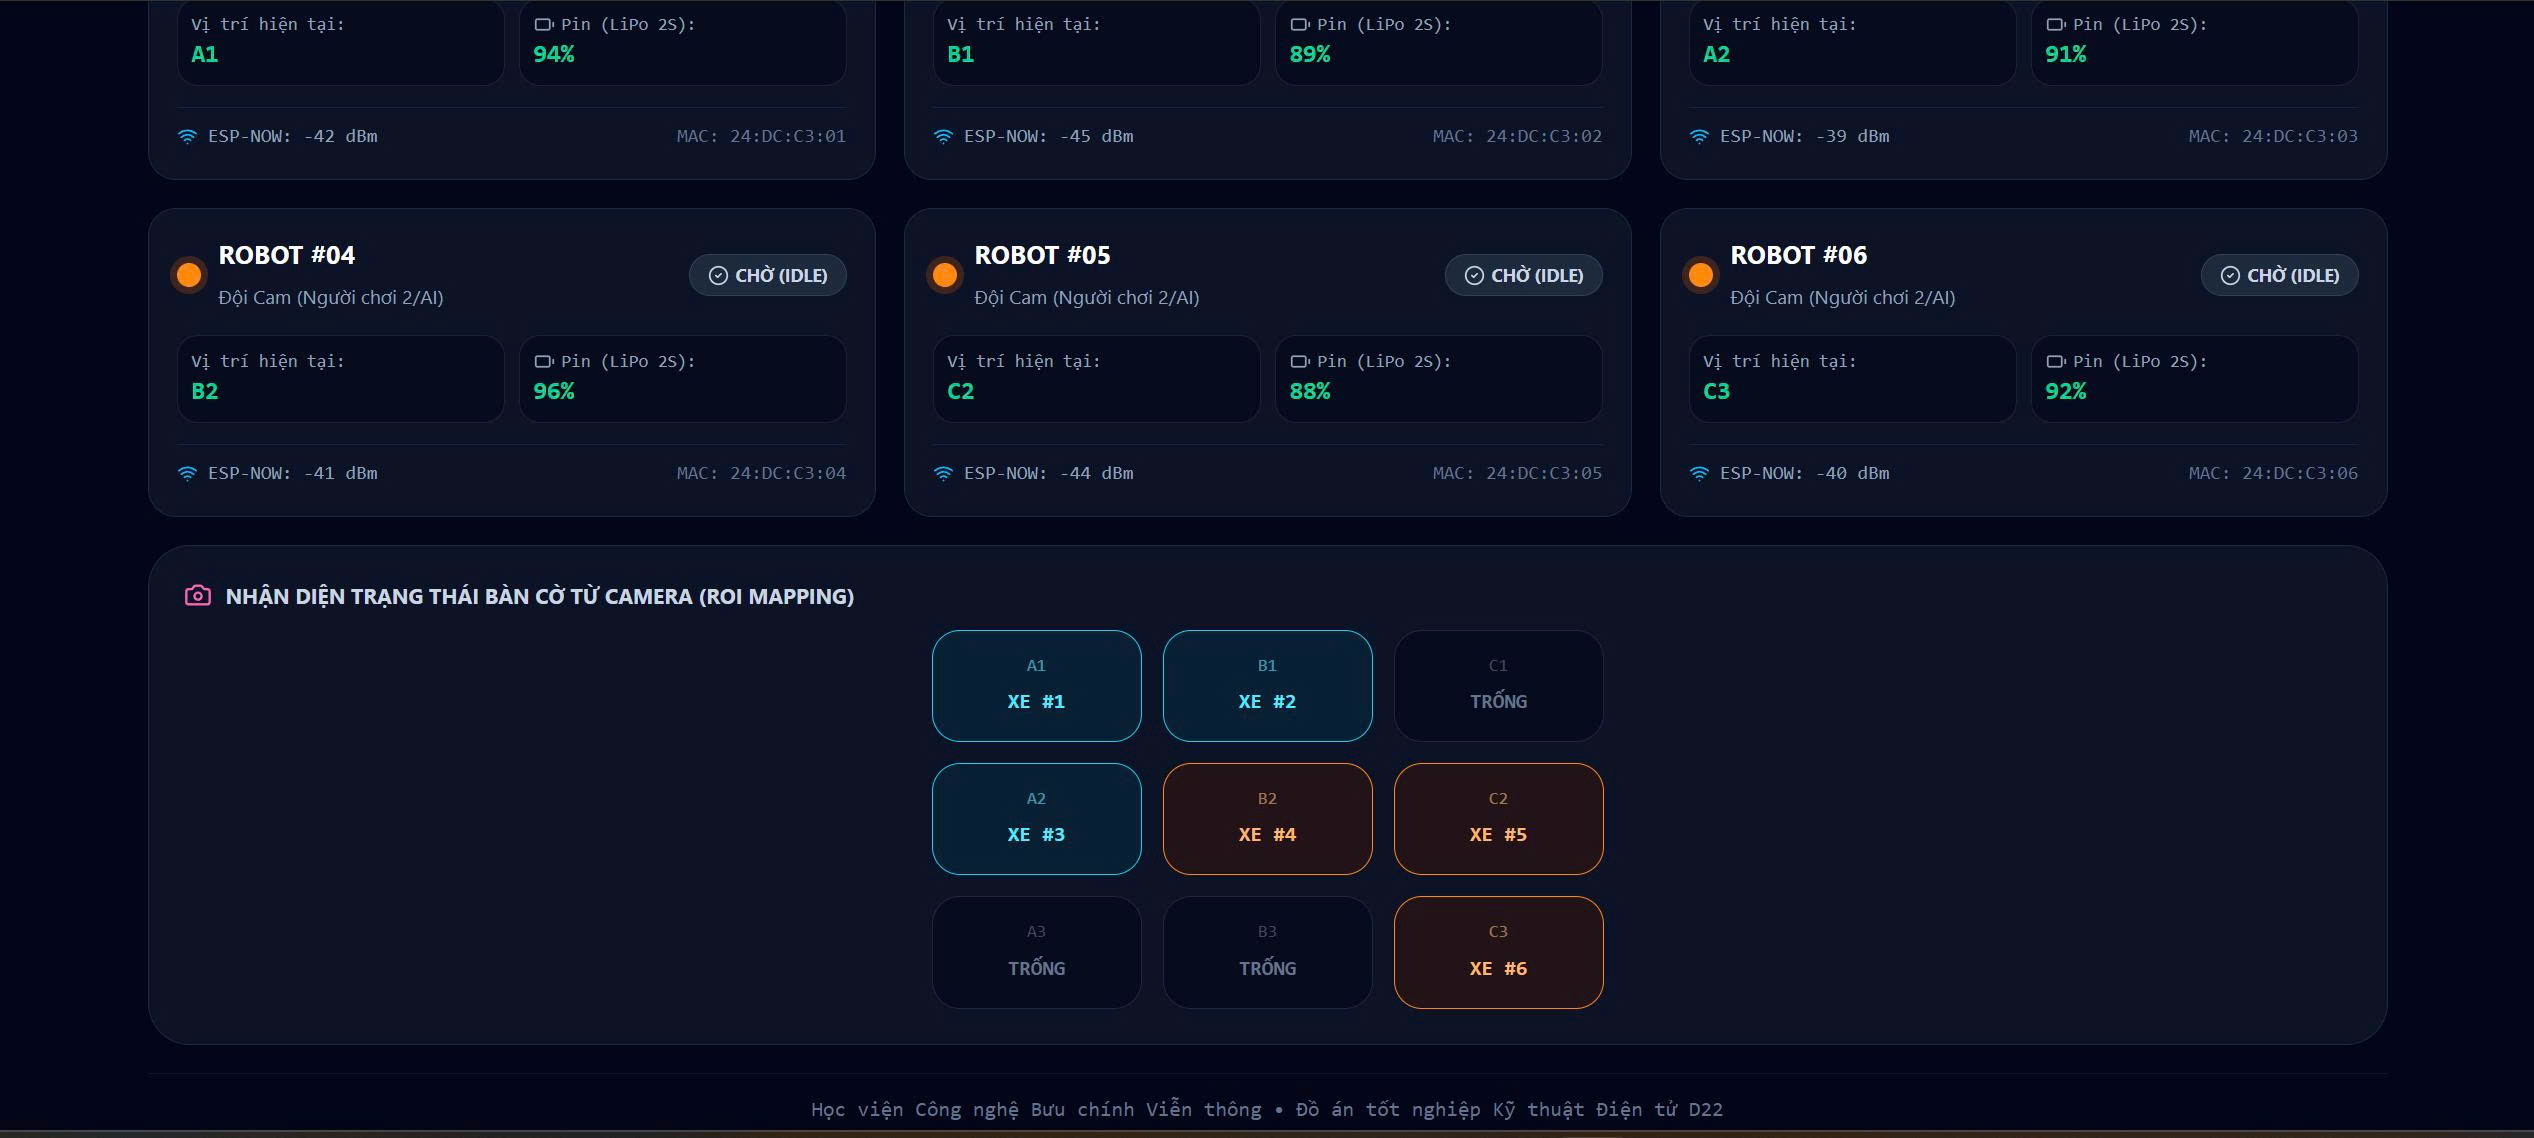
\includegraphics[width=0.95\linewidth]{vitrixe.png}}{\fbox{\parbox[c][4cm][c]{0.8\textwidth}{\centering \itshape \textcolor{red}{[Thiếu file vitrixe.png]}}}}
    \caption{Hiển thị trực quan vị trí và hướng xe trên bàn cờ}
    \label{fig:vitrixe}
\end{figure}
\begin{figure}[H]
    \centering
    \IfFileExists{banco.png}{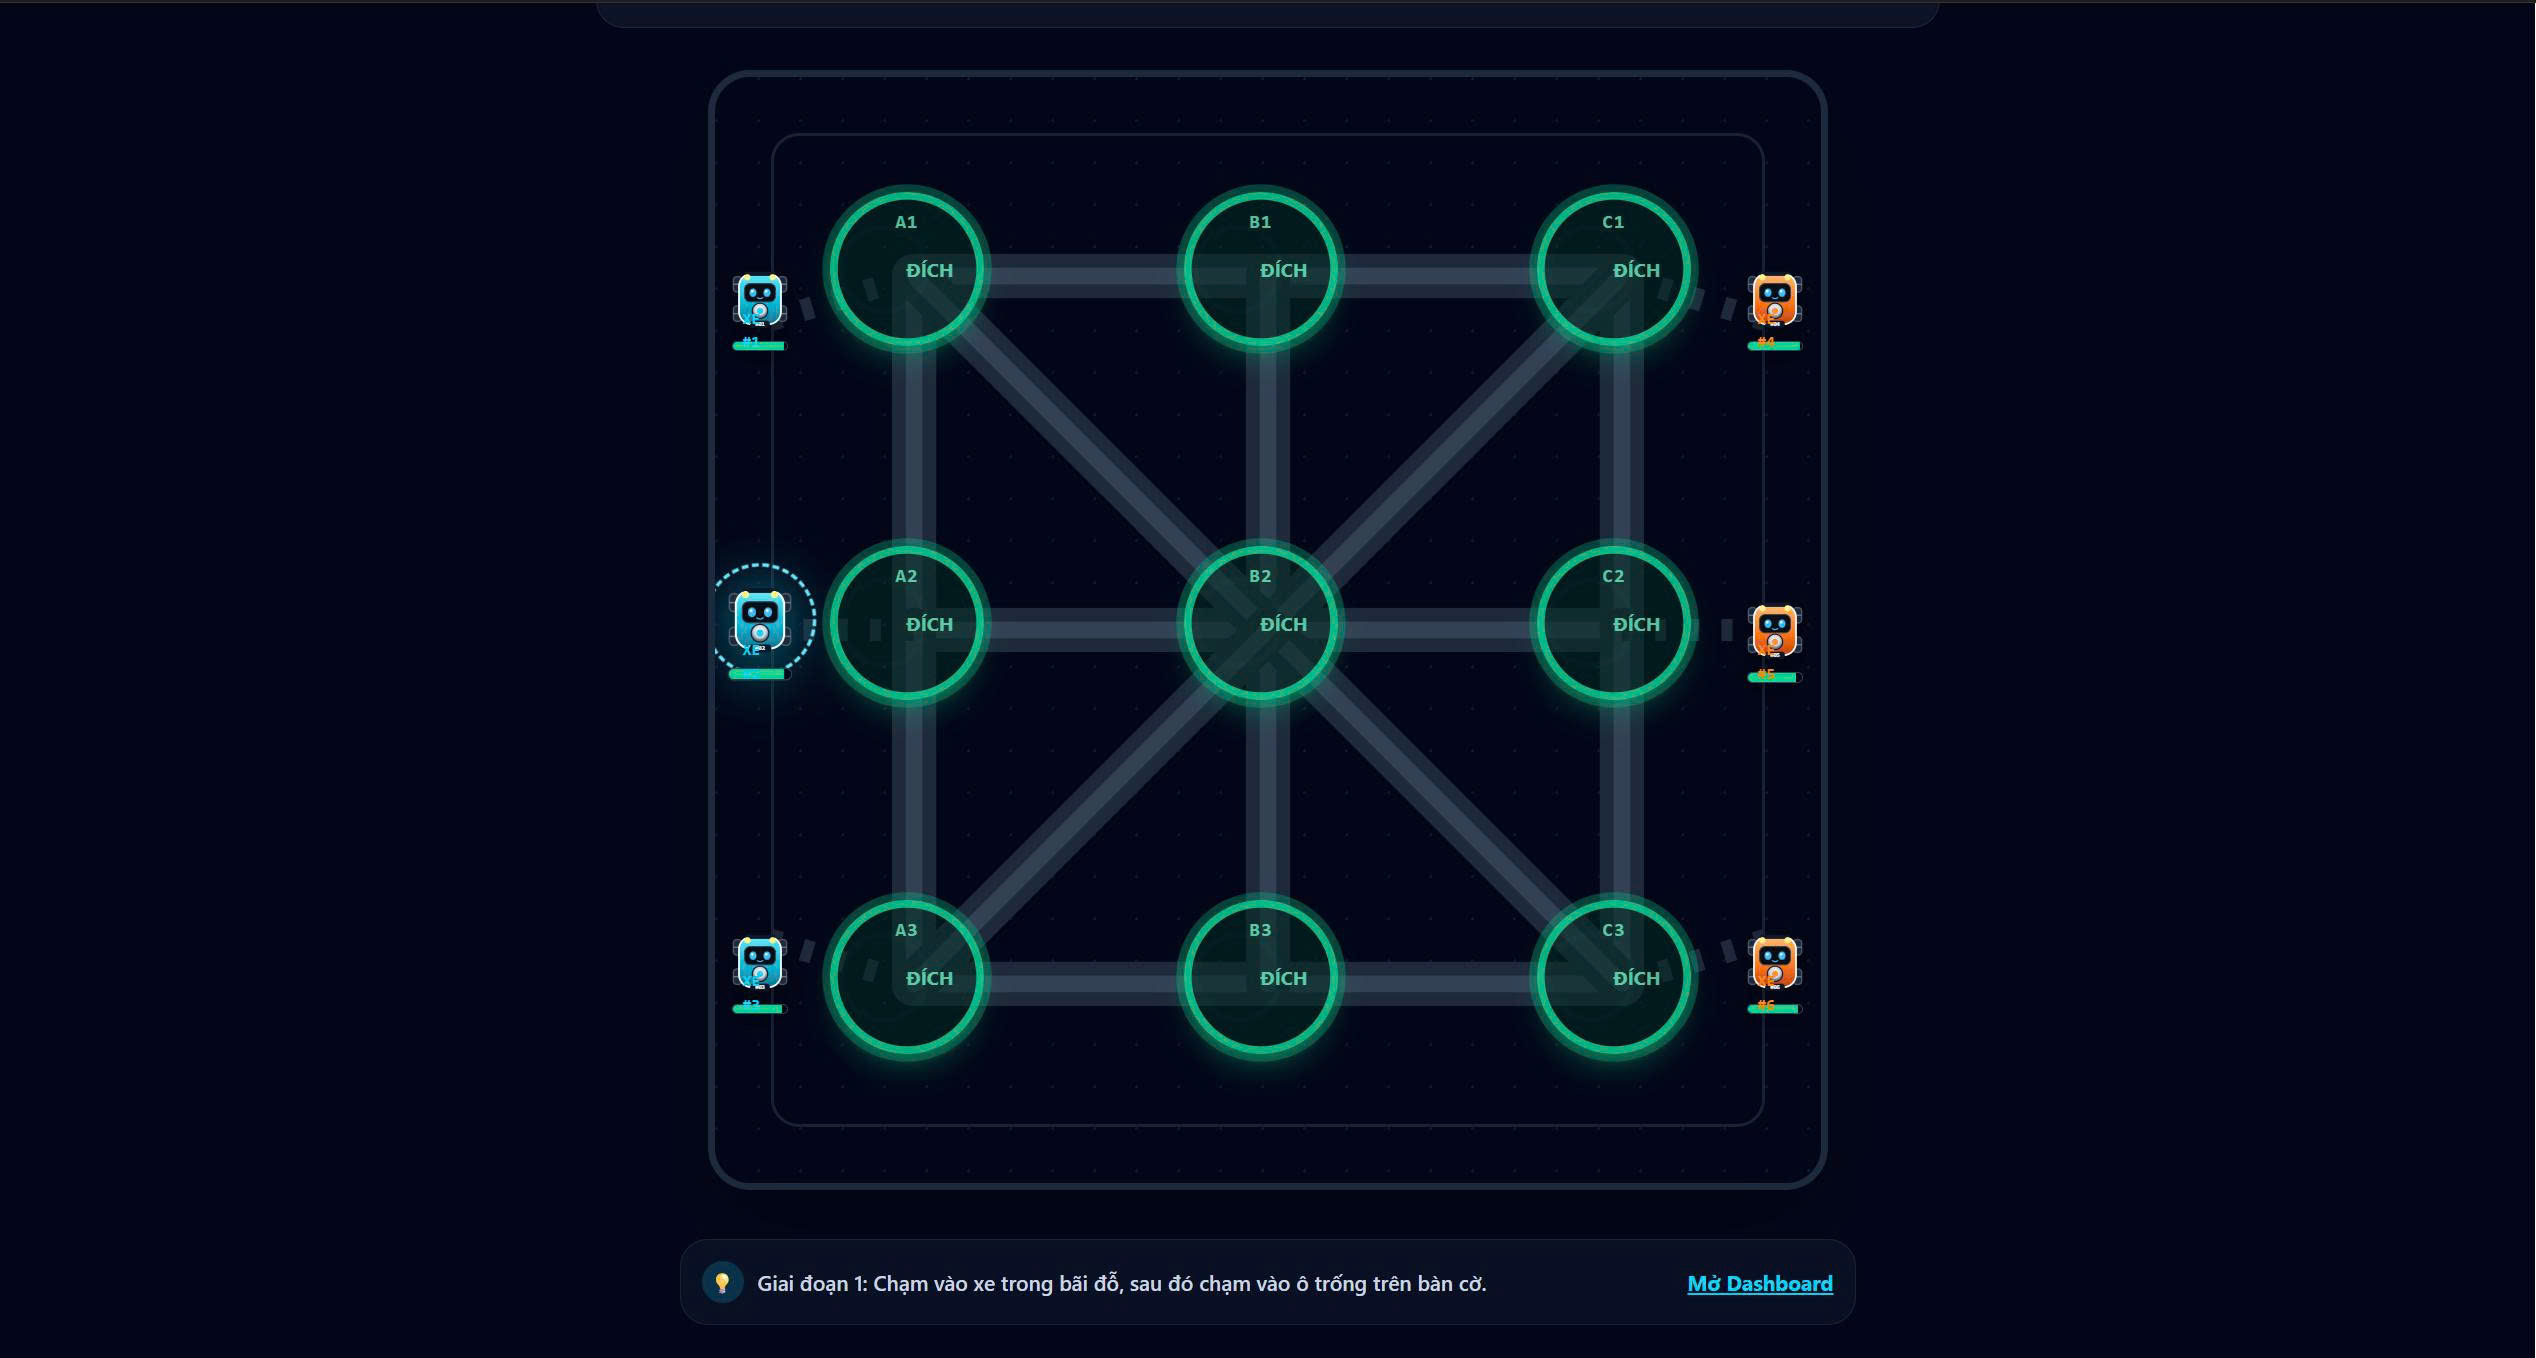
\includegraphics[width=0.95\linewidth]{banco.png}}{\fbox{\parbox[c][4cm][c]{0.8\textwidth}{\centering \itshape \textcolor{red}{[Thiếu file banco.png]}}}}
    \caption{Giao diện tương tác ván đấu Three Men's Morris}
    \label{fig:banco}
\end{figure}
 
\section*{4.6 Lập trình nhúng và hoàn thiện điều khiển chuyển động trên xe}
Nhóm đã hoàn thiện chương trình nhúng (\texttt{code\_xe.ino}, \texttt{drive.cpp}, \texttt{localize.cpp}) trên vi điều khiển ESP32-WROOM-32D. Các khối chức năng điều khiển và cảm biến trên xe đều đã được hiệu chỉnh và hoạt động ổn định:

\begin{table}[H]
\centering
\caption{Kết quả hoàn thiện các khối chức năng nhúng trên xe robot}
\begin{tabular}{L{3.8cm} L{6.2cm} L{4.0cm}}
\toprule
\textbf{Chức năng} & \textbf{Giải pháp kỹ thuật thực hiện} & \textbf{Trạng thái} \\
\midrule
Điều khiển động cơ & Xuất xung PWM 20 kHz điều khiển cầu H DRV8833, có chân kích hoạt nSLEEP chống giật khi khởi động & Hoàn thành, chạy ổn định \\
Định vị góc quay (MPU6050) & Giao tiếp I2C đọc vận tốc góc trục Z, hiệu chỉnh trôi điểm không (gyro bias) và tích phân góc hướng & Hoàn thành, đo góc chính xác \\
Bộ điều khiển PID dò line & Đọc ADC1 mảng 5 cảm biến TCRT5000L học ngưỡng thích nghi, tính sai số vị trí vạch và điều khiển PID lái & Hoàn thành, hết dao động \\
Định vị lai (Odometry) & Kết hợp xung encoder hai bánh và con quay MPU6050 (bộ lọc bù trọng số $\alpha = 0,85$) ở tần số 200 Hz & Hoàn thành \\
Giao tiếp ESP-NOW & Nhận gói lệnh waypoint, điều khiển LED WS2812B và gửi phản hồi trạng thái về Coordinator & Hoàn thành, thông suốt \\
\bottomrule
\end{tabular}
\end{table}

Đặc biệt, sau quá trình hiệu chỉnh các hệ số $K_p, K_i, K_d$ và tốc độ nền PWM, bộ điều khiển \textbf{PID dò line} trên xe đã khắc phục được hiện tượng dao động thân xe khi bám đường thẳng, giữ xe chạy ổn định dọc theo các cạnh của bàn cờ và phát hiện chính xác các nút giao.
 
\begin{figure}[H]
    \centering
    \IfFileExists{pid.png}{\includegraphics[width=0.85\linewidth]{pid.png}}{\fbox{\parbox[c][4cm][c]{0.8\textwidth}{\centering \itshape \textcolor{red}{[Thiếu file pid.png]}}}}
    \caption{Kết quả hiệu chỉnh bộ điều khiển PID dò line ổn định trên xe}
    \label{fig:pid}
\end{figure}
 
% ============================================================
\chapter*{5. KẾ HOẠCH CÔNG VIỆC TIẾP THEO}
\addcontentsline{toc}{chapter}{5. KẾ HOẠCH CÔNG VIỆC TIẾP THEO}
 
Trong giai đoạn tiếp theo (Tuần 10--14), nhóm tập trung ghép nối toàn diện các phân hệ đã hoàn thiện và tối ưu hóa chuyển động thực tế của cụm 6 xe trên bàn cờ:

\begin{table}[H]
\centering
\begin{tabular}{L{5.2cm} c c L{4.8cm}}
\toprule
\textbf{Công việc} & \textbf{Phụ trách} & \textbf{Thời gian} & \textbf{Tiêu chí hoàn thành} \\
\midrule
Kết hợp toàn hệ thống (Camera ArUco -- Minimax -- BFS/A* -- ESP-NOW -- 6 xe) & Cả 2 & Tuần 10--11 & Toàn bộ các tầng giao tiếp khép kín, xe nhận và thực thi đúng nước cờ của AI \\
Tối ưu chương trình di chuyển giữa các vị trí trên bàn cờ và bãi đỗ & Phúc & Tuần 11--12 & Xe quay góc, bám line và giảm tốc dừng tại tâm ô cờ mượt mà, không lệch tâm \\
Kiểm thử kịch bản tránh va chạm và nhường đường đa xe trên sa bàn & Cả 2 & Tuần 12 & Thực hiện trơn tru các tình huống dời xe cản đường trong cả 2 pha của ván đấu \\
Đo đạc thông số thực nghiệm (sai số vị trí, thời gian phản hồi, độ tin cậy) & Cả 2 & Tuần 12--13 & Hoàn thành bảng số liệu đánh giá hiệu năng hệ thống thực tế \\
Hoàn thiện quyển báo cáo ĐATN và chuẩn bị slide bảo vệ trước hội đồng & Cả 2 & Tuần 13--14 & Hoàn tất quyển báo cáo chuẩn định dạng Khoa ĐT1 và sẵn sàng bảo vệ \\
\bottomrule
\end{tabular}
\end{table}
 
% ============================================================
\chapter*{6. KHÓ KHĂN ĐÃ GIẢI QUYẾT VÀ ĐỊNH HƯỚNG TỐI ƯU}
\addcontentsline{toc}{chapter}{6. KHÓ KHĂN ĐÃ GIẢI QUYẾT VÀ ĐỊNH HƯỚNG TỐI ƯU}
 
\section*{6.1 Các vấn đề kỹ thuật đã giải quyết thành công từ lần 1}
\begin{itemize}
    \item \textbf{Chế tạo và ổn định phần cứng cụm 6 xe:} Nhóm đã hoàn thiện toàn bộ mạch in PCB, lắp ráp cơ khí và tách riêng nguồn động lực cho cầu H DRV8833 khỏi nguồn nuôi vi điều khiển ESP32, giúp cả 6 xe hoạt động ổn định, loại bỏ nhiễu nguồn.
    \item \textbf{Khử dao động bộ điều khiển PID dò line:} Thông qua việc chuẩn hóa thuật toán học ngưỡng nền/vạch thích nghi cho 5 cảm biến TCRT5000L và tinh chỉnh bộ tham số PID, xe đã bám đường thẳng mượt mà, không còn hiện tượng lắc ngang.
    \item \textbf{Hiệu chỉnh Camera và đồng bộ góc hướng:} Việc lưu cố định ma trận biến đổi đồng ứng (Homography) từ 4 thẻ ArUco góc bàn cờ giúp triệt tiêu hiện tượng rung khung hình; kết hợp góc phương vị từ ArUco và con quay hồi chuyển MPU6050 cho phép xác định chính xác tư thế và góc hướng của từng xe.
    \item \textbf{Thông suốt truyền thông ESP-NOW:} Áp dụng kiến trúc đa tác vụ FreeRTOS trên ESP32 Coordinator cùng định dạng gói tin nhị phân kích thước nhỏ (8--18 byte) giúp truyền nhận lệnh hai chiều ổn định với các xe.
\end{itemize}

\section*{6.2 Trọng tâm tối ưu trong giai đoạn ghép nối toàn hệ thống}
\begin{itemize}
    \item \textbf{Vấn đề cần tối ưu:} Khi ghép nối toàn hệ thống, mỗi nước đi của xe trên bàn cờ đòi hỏi sự chuyển tiếp liên tục giữa các trạng thái: \textit{xuất phát từ bãi đỗ (không có vạch kẻ) $\rightarrow$ bắt vào đường line bàn cờ $\rightarrow$ quay góc tại nút giao $\rightarrow$ dừng chính xác tại tâm ô đích}. Nếu chuyển pha đột ngột hoặc giảm tốc chưa hợp lý, xe có thể bị trượt quán tính nhẹ làm lệch tâm ô cờ.
    \item \textbf{Giải pháp thực hiện:}
    \begin{enumerate}
        \item Tinh chỉnh hàm giảm tốc tuyến tính theo khoảng cách còn lại tới waypoint kết hợp tín hiệu bắt vạch ngang từ 3 mắt cảm biến hồng ngoại giữa để khóa chính xác tâm nút giao.
        \item Sử dụng tọa độ và góc hướng thực tế từ Camera (ArUco) làm vòng hiệu chỉnh phản hồi sau mỗi bước di chuyển nhằm triệt tiêu hoàn toàn sai số tích lũy của odometry, giúp xe di chuyển giữa các vị trí trên bàn cờ mượt mà và chính xác nhất.
    \end{enumerate}
\end{itemize}
 
% ============================================================

\renewcommand{\bibname}{TÀI LIỆU THAM KHẢO}
\begin{thebibliography}{9}
    \bibitem{tu} Từ Minh Phương, \textit{Giáo trình Trí tuệ nhân tạo}, Học viện Công nghệ Bưu chính Viễn thông, Hà Nội, 2018.
    \bibitem{russell} S. Russell and P. Norvig, \textit{Artificial Intelligence: A Modern Approach}, 4th ed., Pearson, 2020.
    \bibitem{astar} P. E. Hart, N. J. Nilsson, and B. Raphael, ``A formal basis for the heuristic determination of minimum cost paths,'' \textit{IEEE Trans. Syst. Sci. Cybern.}, Vol. 4, No. 2, pp. 100--107, 1968.
    \bibitem{espnow} Espressif Systems, \textit{ESP-NOW User Guide and ESP-IDF Programming Manual}, 2025.
    \bibitem{aruco} S. Garrido-Jurado et al., ``Automatic generation and detection of highly reliable fiducial markers under occlusion,'' \textit{Pattern Recognition}, Vol. 47, No. 6, pp. 2280--2292, 2014.
    \bibitem{siegwart} R. Siegwart, I. R. Nourbakhsh, and D. Scaramuzza, \textit{Introduction to Autonomous Mobile Robots}, 2nd ed., MIT Press, 2011.
\end{thebibliography}
 
\end{document}